\chapter{Nomenclature and Scope of the document}
The document wants to give a basic level guide for the design of IPMSM (interior permanent magnet synchronous machine) using ANSYS RMxprt and ANSYS Maxwell (Electronic).  
\begin{itemize}
	\item[--] The ANSYS toolbox RMxprt will be used to design the PMSM from specifics geometries already available in toolbox.
	\item[--] The ANSYS toolbox Maxwell will be used to perform FEM (finite element method) analysis.
\end{itemize}
\vspace{10mm}
Along the document, the following notation will be used:
\begin{itemize}
	\item[--] RMB : \textit{right mouse button};
	\item[--] LMB : \textit{left mouse button};
	\item[--] DLMB : \textit{double left mouse button};
	\item[--] $\rightarrow$ : \textit{go to}.
\end{itemize}
Moreover, achievements as well as important steps will be marked with a grey box:
\begin{mybox}
	\textbf{e.g.}
\end{mybox}

\chapter{RMxprt Toolbox for IPMSM}
\section{Introduction} 
\textbf{RMxprt} is a ANSYS Electronics toolbox used for the design of different typologies of motors: based on induction principle as well as based on permanent magnets. 

In the following will be considered the design of a synchronous motor based on interior permanent magnet. As case study we design an IPMSM with the following characteristics

\rowcolors{1}{gray!25}{white}
\setlength\arrayrulewidth{1pt}
\begin{center}
	\setlength{\extrarowheight}{6pt}
	\begin{tabular}{m{16em} m{8em} m{8em}}
		\textbf{Rated Power} & \hspace{20mm} & $\SI{200}{\kilo\watt}$ \\[6pt]
		\hspace{5mm}at motor speed & \hspace{20mm} & $\SI{1500}{\per\minute}$ (rpm) \\[6pt]
		\textbf{Rated Torque} & \hspace{20mm} & $\SI{1250}{\newton\meter}$ \\[6pt]
		\hspace{5mm}at motor speed & \hspace{20mm} & $\SI{1500}{\per\minute}$ (rpm) \\[6pt]
		\textbf{Rated Speed} & \hspace{20mm} & \\[6pt]
		\hspace{5mm}maximum motor speed & \hspace{20mm} & $\SI{2140}{\per\minute}$ (rpm) \\[6pt]
		\hspace{5mm}nominal motor speed & \hspace{20mm} & $\SI{1500}{\per\minute}$ (rpm) \\[6pt]
		\textbf{Number of Poles} & \hspace{20mm} & 8\\[6pt]
		\textbf{Number of Slots} & \hspace{20mm} & 12\\[6pt]
	\end{tabular}
	\captionsetup{width=0.5\textwidth}		
	\captionof{table}{PMSM Data as Case Study.}
	\label{motor_data}
\end{center}

%\begin{itemize}
%	\item[--] Nominal Power: \SI{190}{\kilo\watt}.
%	\item[--] Nominal Torque: \SI{1250}{\newton\meter}.
%	\item[--] Nominal Speed: \SI{1500}{\per\minute}.
%	\item[--] Maximum Speed: \SI{2140}{\per\minute}.
%	\item[--] Number of Poles: \SI{8}{}.
%	\item[--] Number of Slots: \SI{12}{}.
%\end{itemize}
\section{Setup of RMxprt design} 
Here, the preliminary steps for the setup of the RMxprt tool design.
\begin{itemize}
	\item[--] From ANSYS Workbench $\rightarrow$ DLMB \textbf{RMxprt}
	\begin{itemize}
		\item[--] From \textit{Project Schematic}-\textit{RMxprt Design} DLMB \textit{setup}.
	\end{itemize} 
	\item[--] From \textbf{RMxprt} $\rightarrow$ \textbf{Project Manager} $\rightarrow$ \textbf{MaxwellProject} $\rightarrow$ RMB on \textbf{RMxprtDesign1} and select: \textit{Machine Type...}
	\item[--] From \textit{Design Flow} select: \textit{Generate RMxprt Solutions}.
	\item[--] From \textit{Machine Type} select: \textit{General}. 
	\item[--] From the bottom window select: \textit{Synchronous Machines} $\rightarrow$ \textit{IPM Synchronous Machine}.
	\item[--] Press OK.
\end{itemize}
\vspace{10mm}
After these preliminary steps, specific icons list will be appeared in the tree of the \textit{RMxprtDesign1}. The following steps shall be done.
\begin{itemize}
	\item[--] LMB on \textit{Machine} and select:
	\begin{table}[H]
		\begin{center}
			\begin{tblr}{
					hlines,
					vlines,
					row{1}={bg=lightgray}
				} 
				Parameter & Input	\\
				Source Type & AC	\\
				Structure & Inner Rotor	\\
				Stator Type & SLOT\_AC	\\
				Rotor Type & PM\_INTERIOR
			\end{tblr}
		\end{center}
		\captionsetup{width=.5\textwidth}
		\caption{Machine setup.}
		\label{msetup_1}
	\end{table}	
\end{itemize}

\begin{itemize}
	\item[--] LMB on \textit{Machine-Stator} and select:
	\begin{table}[H]
		\begin{center}
			\begin{tblr}{
					hlines,
					vlines,
					row{1}={bg=lightgray}
				} 
				Parameter & Input \\
				Number of Poles & 8 \\
				Number of Slots & 12 \\
				Circuit Type & Y3 \\
				Slot Type & 4 \\
				Position Control & unchecked
			\end{tblr}
		\end{center}
		\captionsetup{width=.5\textwidth}
		\caption{Machine-Stator setup.}
		\label{mssetup_1}
	\end{table}	
\end{itemize}


\begin{itemize}
	\item[--] LMB on \textit{Machine-Stator-Core} and select:
	\begin{table}[H]
		\begin{center}
			\begin{tblr}{
					hlines,
					vlines,
					row{1}={bg=lightgray}
				} 
				Parameter & Input \\
				Outer Diameter & \SI{640}{\milli\meter} \\
				Inner Diameter & \SI{450}{\milli\meter} \\
				Length & \SI{160}{\milli\meter} \\
				Stacking Factor & 0.95 \\
				Steel Type & isovac 400 65A \\
				Press Board Thickness & \SI{0}{\milli\meter} \\
				Magnetic Press Board & unchecked \\
				Skew Width & \SI{0}{\degree} \\
				Lamination Sector & \SI{0}{}
			\end{tblr}
		\end{center}
		\captionsetup{width=.5\textwidth}
		\caption{Machine-Stator-Core setup.}
		\label{mscsetup_1}
	\end{table}	
\end{itemize}

\begin{itemize}
	\item[--] LMB on \textit{Machine-Stator-Core-Slot} and select:
	\begin{table}[H]
		\begin{center}
			\begin{tblr}{
					hlines,
					vlines,
					row{1}={bg=lightgray}
				} 
				Parameter & Input \\
				Auto Design & unchecked \\
				Parallel Tooth Design & unchecked \\
				$H_{s0}$ & \SI{6}{\milli\meter} \\
				$H_{s1}$ & \SI{0}{\milli\meter}	\\
				$H_{s2}$ & \SI{55}{\milli\meter} \\
				$B_{s0}$ & \SI{48}{\milli\meter} \\
				$B_{s1}$ & \SI{55}{\milli\meter} \\
				$B_{s2}$ & \SI{55}{\milli\meter} \\	
				$R_{s}$ & \SI{2}{\milli\meter}
			\end{tblr}
		\end{center}
		\captionsetup{width=.5\textwidth}
		\caption{Machine-Stator-Core-Slot setup.}
		\label{mscssetup_1}
	\end{table}	
\end{itemize}

\begin{itemize}
	\item[--] LMB on \textit{Machine-Stator-Winding} and select:
	\begin{table}[H]
		\begin{center}
			\begin{tblr}{
					hlines,
					vlines,
					row{1}={bg=lightgray}
				} 
				Parameter & Input \\
				Winding Layers & 2 \\
				Winding Type & Whole-Coiled \\
				Parallel Branches & 4 \\
				Conductor per Slot & 60 \\
				Coil pitch & 1 \\
				Number of Strands & 0 \\
				Wire Wrap & \SI{0}{\milli\meter} \\
				Wire Size & \SI{0}{\milli\meter} \\
				Conductor Type & Aluminium
			\end{tblr}
		\end{center}
		\captionsetup{width=.5\textwidth}
		\caption{Machine-Stator-Winding setup.}
		\label{mswsetup_1}
	\end{table}	
	\begin{table}[H]
		\begin{center}
			\begin{tblr}{
					hlines,
					vlines,
					row{1}={bg=lightgray}
				} 
				Parameter & Input \\
				Input Half-turn Length & unchecked \\
				End Extension & \SI{0}{\milli\meter} \\
				Correction Factor & 1 \\
				Base Inner Radius & \SI{0}{\milli\meter} \\
				Tip Inner Diameter & \SI{0}{\milli\meter} \\
				End Clearance & \SI{0}{\milli\meter} \\
				Slot Liner & \SI{0}{\milli\meter} \\
				Wedge Thickness & \SI{0}{\milli\meter} \\
				Layer Insulation & \SI{0}{\milli\meter} \\
				Limited Fill Factor & 0.75 \\
				Top Spare Space & 0 \\
				Bottom Spare Space & 0 \\
			\end{tblr}
		\end{center}
		\captionsetup{width=.5\textwidth}
		\caption{Machine-Stator-Winding (End-Insulation) setup.}
		\label{msweisetup_1}
	\end{table}	
\end{itemize}
\begin{mybox}
	At this step is already possible via RMB, on the right view of the motor section, select \textit{Connect all coils} to se the coils connection.
\end{mybox}


\begin{itemize}
	\item[--] LMB on \textit{Machine-Rotor} and select:
	\begin{table}[H]
		\begin{center}
			\begin{tblr}{
					hlines,
					vlines,
					row{1}={bg=lightgray}
				} 
				Parameter & Input \\
				Number of Poles & 8 
			\end{tblr}
		\end{center}
		\captionsetup{width=.5\textwidth}
		\caption{Machine-Rotor setup.}
		\label{mrsetup_1}
	\end{table}	
\end{itemize}

\begin{itemize}
	\item[--] LMB on \textit{Machine-Rotor-Core} and select:
	\begin{table}[H]
		\begin{center}
			\begin{tblr}{
					hlines,
					vlines,
					row{1}={bg=lightgray}
				} 
				Parameter & Input \\
				Outer Diameter & \SI{444}{\milli\meter} \\
				Inner Diameter & \SI{310}{\milli\meter} \\
				Length & \SI{160}{\milli\meter} \\
				Stacking Factor & 0.95		\\
				Steel Type & isovac 400 65A	\\	
				Pole Type & 4
			\end{tblr}
		\end{center}
		\captionsetup{width=.5\textwidth}
		\caption{Machine-Rotor-Core setup.}
		\label{mrcsetup_1}
	\end{table}	
\end{itemize}

\begin{itemize}
	\item[--] LMB on \textit{Machine-Rotor-Core-Pole} and select:
	\begin{table}[H]
		\begin{center}
			\begin{tblr}{
					hlines,
					vlines,
					row{1}={bg=lightgray}
				} 
				Parameter & Input \\
				$D_1$ & \SI{438}{\milli\meter} \\
				$O_1$ & \SI{12}{\milli\meter} \\
				$O_2$ & \SI{24}{\milli\meter} \\
				$B_1$ & \SI{12}{\milli\meter} \\
				$R_{ib}$ & \SI{12}{\milli\meter} \\
				${\mathit{HR}}_{ib}$ & \SI{4}{\milli\meter} \\
				Layers & 1 \\
				Layer Pitch & \SI{0}{\milli\meter} \\
				Magnet Thickness Pitch & \SI{12}{\milli\meter} \\	
				Magnet Width Pitch & \SI{120}{\milli\meter} \\
				Magnet Type & NdFe35
			\end{tblr}
		\end{center}
		\captionsetup{width=.5\textwidth}
		\caption{Machine-Rotor-Core-Pole setup.}
		\label{mrcpsetup_1}
	\end{table}	
\end{itemize}

\begin{itemize}
	\item[--] LMB on \textit{Machine-Shaft} and select:
	\begin{table}[H]
		\begin{center}
			\begin{tblr}{
					hlines,
					vlines,
					row{1}={bg=lightgray}
				} 
				Parameter & Input \\
				Magnetic Shaft & checked \\
				Frictional Loss & \SI{1200}{\watt} \\
				Windage Loss or Power & \SI{0}{\watt} \\
				Reference Speed & \SI{1500}{\per\minute} (rpm)
			\end{tblr}
		\end{center}
		\captionsetup{width=.5\textwidth}
		\caption{Machine-Shaft setup.}
		\label{mshsetup_1}
	\end{table}	
\end{itemize}

\section{Preparation for Maxwell-Analysis of the RMxprt design} 

\begin{itemize}
	\item[--] From \textbf{RMxprtDesign1}-\textit{Analysis} $\rightarrow$ RMB $\rightarrow$ \textit{Add Solution Setup}
	\item[--] From \textit{Add Solution Setup} select:
	\begin{itemize}
		\item[--] From \textit{General}
		\begin{table}[H]
			\begin{center}
				\begin{tblr}{
						hlines,
						vlines,
						row{1}={bg=lightgray}
					} 
					Parameter & Input \\
					Setup Name & Analysis\_1 \\
					Operation Type & Motor \\
					Load Type & Constant Speed \\
					Rated Output Power & \SI{200}{\kilo\watt} \\
					Rated Voltage & \SI{400}{\volt} \\
					Rated Speed & \SI{1500}{\per\minute} (rpm) \\
					Operating Temperature & \SI{75}{\celsius}
				\end{tblr}
			\end{center}
			\captionsetup{width=.5\textwidth}
			\caption{General - Solution setup.}
			\label{g_solution_setup_1}
		\end{table}	
		\item[--] From \textit{Generic Rotating Machine}
		\begin{table}[H]
			\begin{center}
				\begin{tblr}{
						hlines,
						vlines,
						row{1}={bg=lightgray}
					} 
					Parameter & Input \\
					Rated Power Factor & 0.8 \\
					Frequency & \SI{100}{\hertz}
				\end{tblr}
			\end{center}
			\captionsetup{width=.5\textwidth}
			\caption{Generic Rotating Machine - Solution setup.}
			\label{grm_solution_setup_1}
		\end{table}	
	\end{itemize}
\end{itemize}

\begin{mybox}
	\begin{itemize}
		\item[--] To create the solution: 
		\begin{itemize}
			\item[--] RMB $\rightarrow$ \textbf{RMxprtDesign1}-\textit{Analysis}-\textit{Analysis\_1} $\rightarrow$ \textit{Analyze}.
		\end{itemize}
		\item[--] When terminated check \textit{Message Manager}. 
	\end{itemize}
\end{mybox}



\chapter{Maxwell Analysis}
\section{Maxwell 2D Design} 

\begin{itemize}
	\item[--] To create a Maxwell 2D design: RMB $\rightarrow$ \textit{Analysis-Analysis\_1} $\rightarrow$ \textit{Create Maxwell Design} and select
	\begin{itemize}
		\item[--] Type $\rightarrow$ Maxwell 2D Design
		\item[--] Solution Setup $\rightarrow$ Analysis\_1
		\item[--] Press OK
	\end{itemize}
\end{itemize}

\begin{mybox}
	Once Maxwell 2D design is completed via RMB $\rightarrow$ \textit{Maxwell2DDesign1} is possible to select the 
	\begin{itemize}
		\item[--] \textit{Magnetic}
		\begin{itemize}
			\item[--] \textit{Magnetostatic}
			\item[--] \textit{Transient}
		\end{itemize}
	\end{itemize}
	As default is selected the \textit{Transient} analysis.
\end{mybox}


\subsection{Transient Analysis} 
Once the \textbf{Maxwell2DDesign1(Transient,XY)} is completed a validation procedure must be performed. 
\begin{itemize}
	\item[--] From \textit{Simulation} tab select \textit{Validate}: results will show a exclamation mark over \textit{Boundaries and Excitations}. 
\end{itemize}

\begin{mybox}
	To fix the warning follows the steps:
	\begin{itemize}
		\item[--] From drawing window select the stator iron (selected part will appear magenta) $\rightarrow$ RMB $\rightarrow$ \textit{Assign Excitation} - \textit{Set Eddy Effects} and select:
		\begin{itemize}
			\item[--] Use suggested values
		\end{itemize}
		\item[--] From drawing window select the rotor iron (selected part will appear magenta) $\rightarrow$ RMB $\rightarrow$ \textit{Assign Excitation} - \textit{Set Eddy Effects} and select:
		\begin{itemize}
			\item[--] Use suggested values
		\end{itemize}
	\end{itemize}
	Check \textit{Simulation-Validate} again: the warning should be disappeared.
\end{mybox}
\vspace{10mm}

The PMSM is driven by a specific set of symmetric three phase current (amplitude and phase concur in the definition of the torque) which must be properly set in the excitation fields as follows
\begin{itemize}
	\item[--] LMB $\rightarrow$ \textbf{Maxwell2DDesign1(Transient)} 
	$\rightarrow$ \textit{Excitations} $\rightarrow$ \textit{PhaseA}
	\begin{table}[H]
		\begin{center}
			\begin{tblr}{
					hlines,
					vlines,
					row{1}={bg=lightgray}
				} 
				Parameter & Input \\
				Name & PhaseA \\
				Type & Winding Group \\
				Winding Type & Current \\
				IsSolid & Stranded \\
				Current & \texttt{-600*sin(position*4-pi/3)} \\
				Number of Parallel Branches & 4
			\end{tblr}
		\end{center}
		\captionsetup{width=.5\textwidth}
		\caption{PhaseA Excitation setup.}
		\label{phaseA_2Dsetup_1}
	\end{table}	  
\end{itemize}

\begin{itemize}
	\item[--] LMB $\rightarrow$ \textbf{Maxwell2DDesign1(Transient)} 
	$\rightarrow$ \textit{Excitations} $\rightarrow$ \textit{PhaseB}
	\begin{table}[H]
		\begin{center}
			\begin{tblr}{
					hlines,
					vlines,
					row{1}={bg=lightgray}
				} 
				Parameter & Input \\
				Name & PhaseB \\
				Type & Winding Group \\
				Winding Type & Current \\
				IsSolid & Stranded \\
				Current & \texttt{-600*sin(position*4-pi/3-2*pi/3)} \\
				Number of Parallel Branches & 4
			\end{tblr}
		\end{center}
		\captionsetup{width=.5\textwidth}
		\caption{PhaseA Excitation setup.}
		\label{phaseB_2Dsetup_1}
	\end{table}	  
\end{itemize}

\begin{itemize}
	\item[--] LMB $\rightarrow$ \textbf{Maxwell2DDesign1(Transient)} 
	$\rightarrow$ \textit{Excitations} $\rightarrow$ \textit{PhaseC}
	\begin{table}[H]
		\begin{center}
			\begin{tblr}{
					hlines,
					vlines,
					row{1}={bg=lightgray}
				} 
				Parameter & Input \\
				Name & PhaseC \\
				Type & Winding Group \\
				Winding Type & Current \\
				IsSolid & Stranded \\
				Current & \texttt{-600*sin(position*4-pi/3-4*pi/3)} \\
				Number of Parallel Branches & 4
			\end{tblr}
		\end{center}
		\captionsetup{width=.5\textwidth}
		\caption{PhaseA Excitation setup.}
		\label{phaseC_2Dsetup_1}
	\end{table}	  
\end{itemize}
\begin{mybox}
	To run the simulation: \textit{Simulation} $\rightarrow$ \textit{Analyze All}
\end{mybox}



\subsection{Magnetostatic Analysis} 
To perform a magnetostatic analysis:
\begin{itemize}
	\item[--] Create a new Maxwell 2D design: RMB $\rightarrow$ \textit{Analysis-Analysis\_1} $\rightarrow$ \textit{Create Maxwell Design} and select
	\begin{itemize}
		\item[--] Type $\rightarrow$ Maxwell 2D Design
		\item[--] Solution Setup $\rightarrow$ Analysis\_1
		\item[--] Press OK
	\end{itemize}
\end{itemize}
When terminated RMB over \textbf{Maxwell2DDesign2(Transient, XY)} and select
\begin{itemize}
	\item[--] Magnetic: Magnetostatic
	\item[--] Press OK
\end{itemize}
\begin{mybox}
	\textbf{Maxwell2DDesign2(Transient, XY)} $\rightarrow$ \textbf{Maxwell2DDesign2(Magnetostatic, XY)}
\end{mybox}

\vspace{10mm}

From \textbf{Maxwell2DDesign2(Magnetostatic, XY)} - \textit{Analysis} RMB \textit{Add Solution Setup}
\begin{table}[H]
	\begin{center}
		\begin{tblr}{
				hlines,
				vlines,
				row{1}={bg=lightgray}
			} 
			Parameter & Input \\
			Name & Magnetostatic\_analysis\_1 \\
		\end{tblr}
	\end{center}
	\captionsetup{width=.5\textwidth}
	\caption{Magnetostatic solution setup.}
	\label{magnetostatic_solution_setup_1}
\end{table}	  
\begin{itemize}
	\item[--] Select via LMB select the rotor iron as well as the stator iron
	\item[--] From \textit{Field Overlays} select \textit{field}-\textit{B}-\textit{Mag\_B}
	\item[--] From \textit{Create Field Plot} select \textit{Mag\_B}-\textit{Stator} and  \textit{Mag\_B}-\textit{Rotor}
	\item[--] uncheck \textit{Full Model}
\end{itemize}
\begin{itemize}
	\item[--] Select via LMB select the rotor iron as well as the stator iron
	\item[--] From \textit{Field Overlays} select \textit{field}-\textit{A}-\textit{Flux Lines}
	\item[--] From \textit{Create Field Plot} select \textit{Flux Lines}-\textit{Stator} and  \textit{Flux Lines}-\textit{Rotor}
	\item[--] uncheck \textit{Full Model}
\end{itemize}

\begin{mybox}
	\begin{itemize}
		\item[--] Validate 
		\item[--] Analyze All
	\end{itemize}
\end{mybox}
Simulation will results as shown in Figure
\begin{figure}[H]
	\centering
	\includegraphics[width = 275pt, angle = 0, keepaspectratio]{figures/ANSYS_tutorial/magnetostatic_result_1.eps}
	\captionsetup{width=0.5\textwidth}		
	\caption{Magnetostatic analysis result.}
	\label{msanalysis_result_1}
\end{figure}
\section{Maxwell 3D Design} 

\begin{itemize}
	\item[--] To create a Maxwell 3D design: RMB $\rightarrow$ \textit{Analysis-Analysis\_1} $\rightarrow$ \textit{Create Maxwell Design} and select
	\begin{itemize}
		\item[--] Type $\rightarrow$ Maxwell 3D Design
		\item[--] Solution Setup $\rightarrow$ Analysis\_1
		\item[--] Press OK
	\end{itemize}
\end{itemize}

When 3D model has been performed, the following steps shall be followed
\begin{itemize}
	\item[--] Check \textit{Simulation}-\textit{Validation}
	\begin{itemize}
		\item[--] From drawing window select the stator iron $\rightarrow$ RMB $\rightarrow$ \textit{Assign Excitation} - \textit{Set Eddy Effects} and select:
		\begin{itemize}
			\item[--] Use suggested values
		\end{itemize}
		\item[--] From drawing window select the rotor iron $\rightarrow$ RMB $\rightarrow$ \textit{Assign Excitation} - \textit{Set Eddy Effects} and select:
		\begin{itemize}
			\item[--] Use suggested values
		\end{itemize}
	\end{itemize}
\end{itemize}

\begin{itemize}
	\item[--] Check \textit{Simulation}-\textit{Validation}
\end{itemize}

\subsection{Transient Analysis} 
From 3D Maxwell design is possible to perform transient analysis, as follows
\begin{itemize}
	\item[--] LMB $\rightarrow$ \textbf{Maxwell3DDesign1(Transient)} 
	$\rightarrow$ \textit{Excitations} $\rightarrow$ \textit{PhaseA}
	\begin{table}[H]
		\begin{center}
			\begin{tblr}{
					hlines,
					vlines,
					row{1}={bg=lightgray}
				} 
				Parameter & Input \\
				Name & PhaseA \\
				Type & Winding Group \\
				Winding Type & Current \\
				IsSolid & Stranded \\
				Current & \texttt{-600*sin(position*4-pi/3)} \\
				Number of Parallel Branches & 4
			\end{tblr}
		\end{center}
		\captionsetup{width=.5\textwidth}
		\caption{PhaseA Excitation setup.}
		\label{phaseA_3Dsetup_1}
	\end{table}	  
\end{itemize}

\begin{itemize}
	\item[--] LMB $\rightarrow$ \textbf{Maxwell3DDesign1(Transient)} 
	$\rightarrow$ \textit{Excitations} $\rightarrow$ \textit{PhaseB}
	\begin{table}[H]
		\begin{center}
			\begin{tblr}{
					hlines,
					vlines,
					row{1}={bg=lightgray}
				} 
				Parameter & Input \\
				Name & PhaseB \\
				Type & Winding Group \\
				Winding Type & Current \\
				IsSolid & Stranded \\
				Current & \texttt{-600*sin(position*4-pi/3-2*pi/3)} \\
				Number of Parallel Branches & 4
			\end{tblr}
		\end{center}
		\captionsetup{width=.5\textwidth}
		\caption{PhaseA Excitation setup.}
		\label{phaseB_3Dsetup_1}
	\end{table}	  
\end{itemize}

\begin{itemize}
	\item[--] LMB $\rightarrow$ \textbf{Maxwell3DDesign1(Transient)} 
	$\rightarrow$ \textit{Excitations} $\rightarrow$ \textit{PhaseC}
	\begin{table}[H]
		\begin{center}
			\begin{tblr}{
					hlines,
					vlines,
					row{1}={bg=lightgray}
				} 
				Parameter & Input \\
				Name & PhaseC \\
				Type & Winding Group \\
				Winding Type & Current \\
				IsSolid & Stranded \\
				Current & \texttt{-600*sin(position*4-pi/3-4*pi/3)} \\
				Number of Parallel Branches & 4
			\end{tblr}
		\end{center}
		\captionsetup{width=.5\textwidth}
		\caption{PhaseA Excitation setup.}
		\label{phaseC_3Dsetup_1}
	\end{table}	  
\end{itemize}

\textbf{START A TRANSIENT ANALYSIS} - to start a transient analysis, the following preliminary steps are required
\begin{itemize}
	\item[--] RMB $\rightarrow$ \textbf{Maxwell3DDesign1(Transient)} and select
	\begin{itemize}
		\item[--] \textit{Validation Check}	(all fields must be checked)
		\item[--] \textit{Analyze All} (simulation will start)
	\end{itemize}
\end{itemize}

\begin{figure}[H]
	\centering
	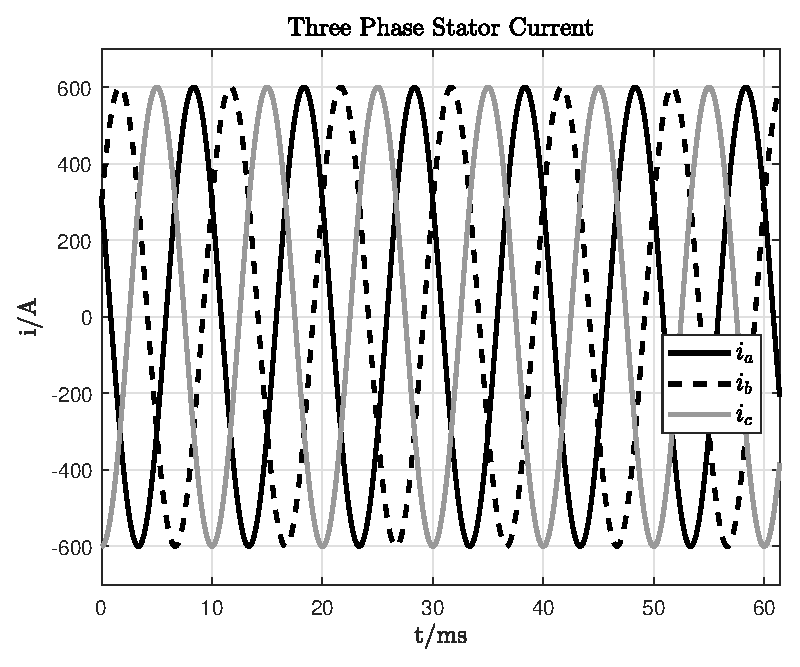
\includegraphics[width = 275pt, angle = 0, keepaspectratio]{figures/ANSYS_tutorial/data3.eps}
	\captionsetup{width=0.5\textwidth}		
	\caption{Simulation results: stator currents.}
	\label{sim_results_3}
\end{figure}
\begin{figure}[H]
	\centering
	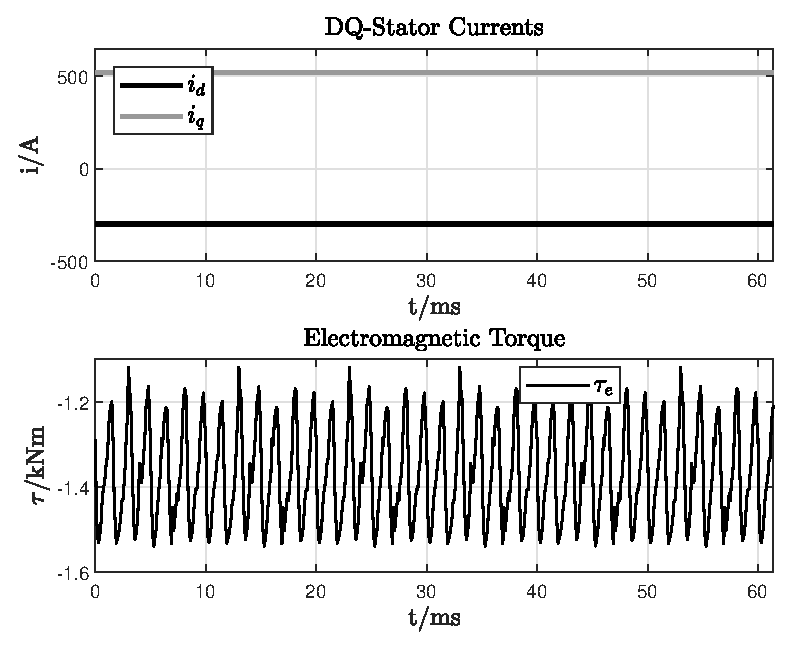
\includegraphics[width = 275pt, angle = 0, keepaspectratio]{figures/ANSYS_tutorial/data1.eps}
	\captionsetup{width=0.5\textwidth}		
	\caption{Simulation results: DQ-Stator currents and electromagnetic torque.}
	\label{sim_results_1}
\end{figure}
\begin{figure}[H]
	\centering
	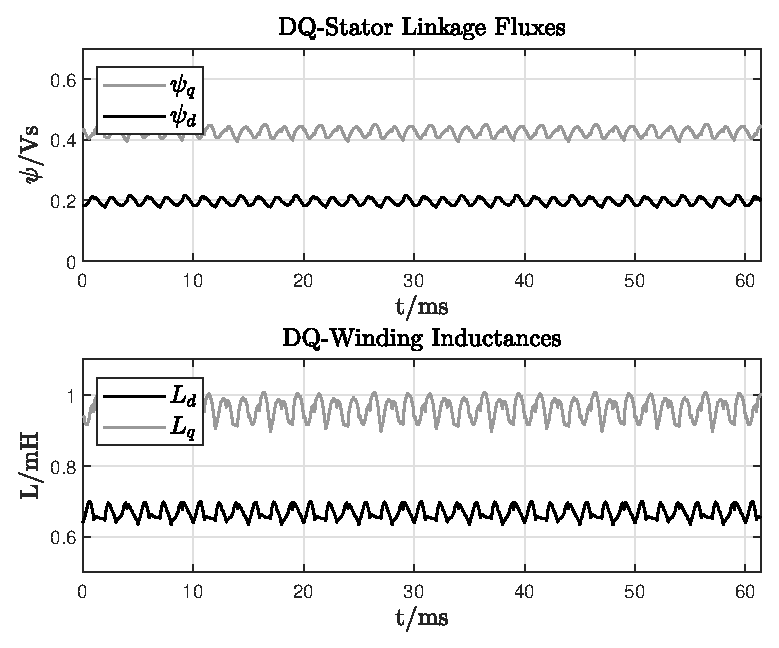
\includegraphics[width = 275pt, angle = 0, keepaspectratio]{figures/ANSYS_tutorial/data2.eps}
	\captionsetup{width=0.5\textwidth}		
	\caption{Simulation results: DQ-fluxes and DQ-inductances.}
	\label{sim_results_2}
\end{figure}

